\section{Aufbau: Erweiterung der Filterkombinationen}
\thispagestyle{fancy}

Im Zuge dieser Arbeit wurden für eine Erhöhung der Messpunkte und Verringerung von Rauschen bei der leistungsdichteabhängigen Messung der IQE die Anzahl der Filterkombination erhöht. Dafür wurden die alten zwei Filterräder durch drei neue ersetzt. 
%
\begin{figure}[ht!]
    \centering
    \begin{minipage}[t]{1\linewidth}
        \centering
        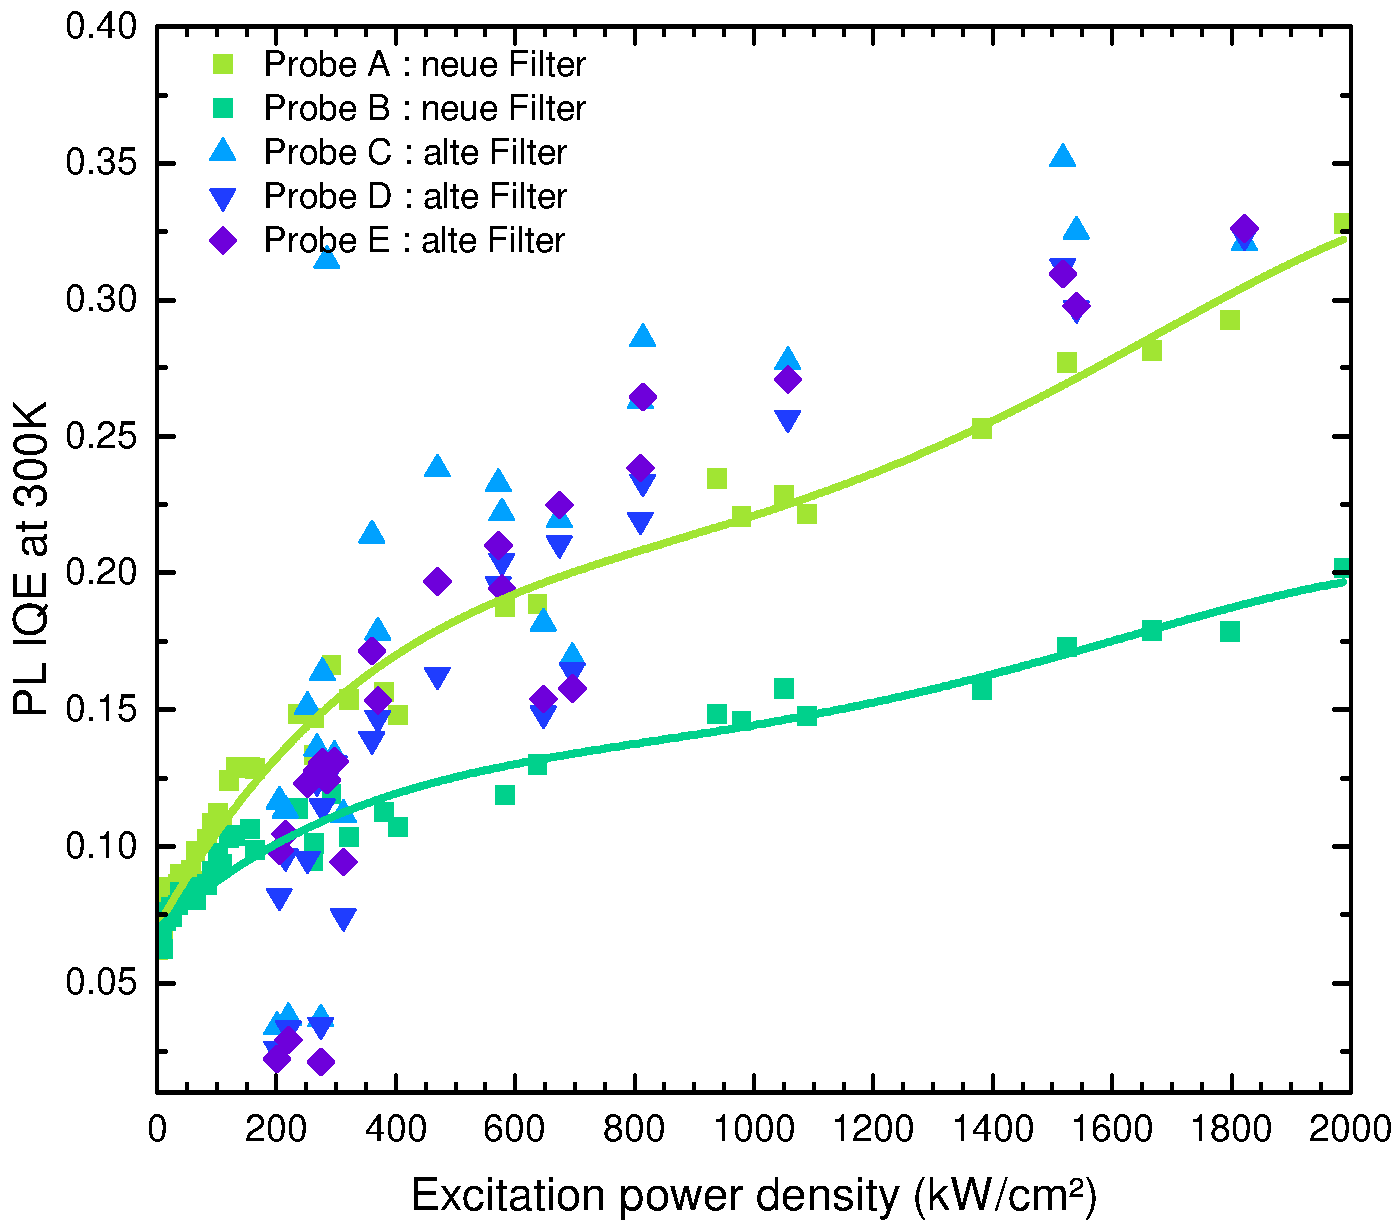
\includegraphics[width = 0.49\linewidth]{Bilder/AuswertungNovemeberKorr1VergleichFilter.pdf}
        \caption{Vergleich der Messung von insgesamt 5 ähnlichen Proben. 3 Proben (blau) wurden mit dem alten Setup gemessen. 2 Proben (grün, durchgezogene Linie) wurden mit dem neuen Setup gemessen. Die Präzision in tieferen Anregungsleistungsdichtenbereichen ist für das neue Setup deutlich erhöht. Das Rauschen fällt ebenfalls deutlich geringer aus. }
        \label{fig:vergleichFilter}
    \end{minipage}
\end{figure}
%
\newpage
Durch die erhöhte Anzahl möglicher Filterkombinationen ist es möglich, statt nur 27 verschiedene Messpunkte 61 zu nehmen. Speziell der Bereich der geringen Anregungsleistungsdichten kann so besser aufgelöst werden und das Rauschen wurde im Allgemeinen stark verringert \ref{fig:vergleichFilter}. 
%
